\documentclass[12pt]{article}

\usepackage{enumitem}
\usepackage[right=20mm, left=20mm]{geometry}
\usepackage{type1cm}
\usepackage{amssymb}
\usepackage[fleqn]{amsmath}
\usepackage{tikz}
\usepackage{multicol}
\usepackage{makecell}
\setlength{\columnsep}{1pt}
\usepackage{pgfplots}
\usepackage{float}
\usepackage{caption}
\usepackage{subcaption}
% \usepackage{subfig}
\usepackage{graphicx}

\usepackage{indentfirst}
\usepackage{lastpage}  
\usepackage{fancyhdr}
\pagestyle{fancy}

\usepackage{pgfgantt}

\usepackage[unicode=true,pdfusetitle,
 bookmarks=true,bookmarksnumbered=false,bookmarksopen=false,
 breaklinks=false,pdfborder={0 0 1},backref=false,colorlinks=false]
 {hyperref}

\makeatletter
\newenvironment{myalign*}{\ifvmode\else\hfil\null\linebreak\fi
  \hspace*{-\leftmargin}\minipage\textwidth
  \setlength{\abovedisplayskip}{0pt}%
  \setlength{\abovedisplayshortskip}{\abovedisplayskip}%
  \start@align\@ne\st@rredtrue\m@ne}%
{\endalign\endminipage\linebreak}

% Paper size
\topmargin -10mm
\textwidth 170mm
% \oddsidemargin -5mm
% \evensidemargin -5mm
\textheight 220mm

% Font setting
\usepackage{xeCJK}
% \setCJKmainfont{Noto Sans TC}
\setCJKmainfont{kaiu.ttf}


\renewcommand{\footnotesize}{\normalsize} 
\renewcommand{\headrulewidth}{0pt}
\renewcommand{\footrulewidth}{0pt}

\lhead{}
\chead{2023年全國大專校院智慧創新暨跨域整合創作企劃書}
\rhead{}

\lfoot{}
\cfoot{}
\rfoot{ 共 \pageref{LastPage} 頁 第  \thepage   頁} 

\makeatletter
\begin{document}
% \fontsize{14pt}{18pt}\selectfont
% \author{}
\date{}
\usetikzlibrary{automata, positioning, arrows}
% \maketitle
\tikzset{every state, accepting/.style={double distance=2pt}}
\captionsetup[figure]{labelfont={bf},name={圖},labelsep=period}

\noindent
\textbf{參賽隊名:} 普羅程式 \\
\textbf{作品名稱:} 威力導師 PowerTeacher \\

\begin{enumerate}
  \setlength{\parindent}{2em}
  \item 競賽主題:數位永續科技組 
  \item 創作主題
    \begin{enumerate}
      \setlength{\parindent}{2em}
      \item 題目
        \par 威力導師 PowerTeacher
      \item 實用功能描述
        \par 在台灣,資訊科技領域備受關注,且程式設計已成為學校必修課程。儘管每年有數百萬學生修習程式課程,但基層教育仍面臨著許多問題:以往的教學方式需頻繁切換畫面給學生練習、課堂上教師無法即時得知學生狀況。所以我們建立一個名為 PowerTeacher 的網頁應用,專注於教師導向的程式教學工具,整合直播、實作、測驗、互動與AI輔助,讓所有人都能進行優質的程式教學。
        \par PowerTeacher 是專為教師設計的教學工具,採網頁應用形式,主要提供三種頁面:
        \begin{enumerate}[label=(\arabic*)]
          \item 學生課堂頁面:學生的學生課堂頁面,有直播區、互動區、功能區(見圖x)。
            \begin{itemize}
              \item 直播區:用於顯示章節投影片,會在課中展示與老師相同的投影片畫面,並同步老師的滑鼠軌跡、繪畫等。
              \item 互動區:用於顯示滾動式的講義,講義可以放文字、圖片、課堂習題,並且在課中,具有引導功能,會根據老師目前的上課投影片,用黃色框線在講義中顯示其對應的位置。
              \item 功能區:用於控制直播區的內容,在課中能夠切換投影片、一鍵回到老師的直播投影片等。在課後能夠拖動時間軸,回放過去的上課直播。
            \end{itemize}
          \item 教師課堂頁面:教師的課堂頁面,與學生的課堂頁面相同,同樣有直播區、互動區、功能區,但功能有部分差異(見圖x)。
            \begin{itemize}
              \item 直播區:用於顯示章節投影片,在課中會將畫面同步到學生的直播區中。
              \item 互動區:用於顯示滾動式講義,並能夠預覽課堂習題的作答統計。
              \item 功能區:用於控制直播功能,能夠開啟與關閉直播,在課中可以切換投影片、切換成畫筆功能等。
            \end{itemize}
          \item 教師講義編輯頁面:
          教師的講義編輯頁面,用於編輯互動區講義的內容,我們將整個講義分為各種不同類型的小區塊,透過將不同類型的區塊做拼接,以完成整個講義。這個構想是參考影片剪輯軟體,能夠在時間軸上,將各個影音片段組合成一部影片。分為編輯區與時間軸(見圖x):
            \begin{itemize}
              \item 編輯區:在右半部點擊不同類型的講義區塊,如文字、選擇題、程式題,就能夠在左半部編輯其中的內容。
              \item 腳本區:下半部的時間軸,用於將不同類型的講義小區塊做不同順序的拼接,以完成整個講義。時間軸的單位是投影片的頁數,讓投影片能對應到不同的講義區塊,在課中就能根據投影片的頁數在講義上做引導與提示。
            \end{itemize}
        \end{enumerate}
      \item 作品與市場相關產品差異
        \par 經過與大學與高中程式教師的實地訪談,我們整理出以下三個時間段的教學流程:
        \begin{enumerate}[label=(\arabic*)]
          \setlength{\parindent}{2em}
          \item 課前:準備教材
            \par 在教學前,教師會準備課堂所需的講義與投影片。市場上的講義編輯功能通常是基於文件編輯器或投影片的形式,例如 Microsoft Word 、Power Point。然而這些工具的功能較為單一,沒辦法嵌入程式執行區、互動習題等與教學相關的功能。我們的平台提供滾動式講義,搭配程式執行、引導、互動習題等功能,使講義內容與課堂做連結。並使用教師講義編輯頁面,使講義更為直觀、易於操作和修改。
          \item 課中:互動教學
            \begin{itemize}
              \item 直播功能:實現直播教學的方式,能大致分為硬體與軟體,硬體上常見的有廣播與管理系統,能夠強制控制學生的畫面。軟體上則有 Zoom、Google Meet 等以視訊為主的會議平台或專為學校開發的遠端控制系統,透過網路分享教師的語音與畫面。這些工具分別有幾項問題:前者是強制控制學生電腦,無法讓學生在課堂中與老師同步實作,也無法用電腦查詢資料、觀看講義等。後者是直播的影音可能有延遲,會導致老師的教學與控制不流暢。我們的特色是讓學生能夠在課堂中,操控投影片回顧上課內容,還能同時觀看補充講義、實作程式碼、回答習題等,讓學生就算在課堂中也能回顧與實作,並以更低延遲的直播投影片取代影像直播,使學習更為流暢。
              \item 引導功能:如何讓學生在課堂中更有參與感並且理解教學內容。市場上的一般教學軟體或平台通常缺乏對於學生學習的引導功能。我們的平台嘗試解決這個問題,透過互動區的黃色框線,在講義中顯示對應的位置,讓學生能夠清楚知道老師目前講解的內容與講義之間的對應。這樣的引導功能可以讓學生更容易理解並隨著教學進度進行,同時也能在回顧時更加方便。
            \end{itemize}
          \item 課後:課程回顧
            \par 在市場上,許多教學平台提供課後回放功能,讓學生能夠在課程結束後回顧老師的教學內容。我們的平台也提供了這樣的功能,讓學生能夠在課後拖動時間軸,回放過去的上課直播,以便進一步學習和復習。不過,我們的特色在於,課後回放不僅僅限於觀看直播畫面,還能夠觀看補充講義、實作程式碼等,並搭配引導功能,讓學生在回顧時更為全面與深入。
        \end{enumerate}
      \par 綜合以上幾點,我們整理了老師上課時可能會用到的工具並做比較:
        \begin{table}[htb]      
          \centering
          \begin{tabular}{|c|c|c|c|c|c|}
            \hline
            \thead{功能} & \thead{本系統} & \thead{Google Meet} & \thead{遠端控制系統} & \thead{CodingBar}  & \thead{廣播與管理系統}\\ \hline
            直播延遲 & 低 & 高 & 高 & 高 & 低 \\ \hline
            教學方式\footnotemark[1] & 線上與實體皆可 & 線上 & 實體 & 線上 & 實體 \\ \hline
            電腦控制 &  &  & 遠端控制\footnote[2] &  & 完全控制 \\ \hline
            課後回顧 & \checkmark &  &  & \checkmark &  \\ \hline
            線上練習\footnote[3] & \checkmark &  &  & \checkmark &\\ \hline
            教學功能整合\footnote[4] & \checkmark &  &  & \checkmark &\\ \hline
          \end{tabular}
          \caption{老師上課時可能會用到的工具比較}
        \end{table}
      \par 本系統在直播延遲、教學方式、課後回顧、線上練習以及教學功能整合方面表現出色,並減少對學生電腦的控制,提供了較佳的教學彈性和互動。
    \end{enumerate}
    
    \footnotetext[1]{教學方式:教學方式分為線上與實體教學,線上教學指的是在網路平台上進行的教學活動,通常包括遠距視訊教學、線上課程和互動學習模式。實體教學指的是在實際的物理教室或學習環境中進行的教學活動,教師與學生面對面進行互動和知識傳遞。}
    \footnotetext[2]{遠端控制:遠端操作是指教師可以強制操作學生的電腦,或者同時與學生在同一台電腦上進行操作。}
    \footnotetext[3]{線上練習:線上練習是指讓學生能夠在線上環境中進行練習、測試和應用所學的知識或技能。這種方式可以包括線上測驗、程式撰寫與評測等。}
    \footnotetext[4]{教學功能整合:教學功能整合是指將不同的教學元素、工具和方法結合在一起,可以是教學資源、互動工具、直播平台等。}
    \item 創意構想
    \begin{enumerate}
      \item 理論基礎
      \item 設計創新說明
      \item 特殊功能描述
    \end{enumerate}
  \item 系統架構
    \begin{enumerate}
      \item 架構說明
      \item 「人機介面設計」(UI)與「使用者體驗」(UX)設計
    \end{enumerate}
  \item 計劃管理
    \begin{table}[htb]      
      \centering
      \begin{tabular}{|c|c|c|}
        \hline
        \thead{工作階段} & \thead{工作日數} & \thead{工作內容} \\ \hline
        1 &  &  \\ \hline
      \end{tabular}
      \caption{計劃管理}
    \end{table}
    \begin{figure}[htb]
      \centering
      \begin{ganttchart}[
        y unit title=0.6cm,
        y unit chart=0.7cm,
        x unit=0.7cm,
        vgrid,hgrid, 
        title height=1,
        progress label text={},
        bar height=0.8,
        bar top shift=0.1,
        ]{1}{8}
        %labels
        \gantttitle{1}{1} 
        \gantttitle{2}{1} 
        \gantttitle{3}{1} 
        \gantttitle{4}{1} 
        \gantttitle{5}{1}
        \gantttitle{6}{1}
        \gantttitle{7}{1}
        \gantttitle{8}{1} \\
        
        %tasks
        \ganttbar{工作階段 1}{1}{2} \\
        \ganttbar{工作階段 2}{3}{4} \\
        \ganttbar{工作階段 3}{5}{6} \\
        \ganttbar{工作階段  4}{7}{8}
        % \ganttbar[progress=0]{工作階段  4}{7}{8}
      
        %relations 
        % \ganttlink{elem0}{elem1} 
      \end{ganttchart}
      \caption{甘特圖}  
    \end{figure}
  \item 修改舊作參賽說明
    \par 本專案開發之作品未使用團隊成員曾獲競賽獎勵之作品。
  \item 軟體清單
    \begin{enumerate}
      \item 作業系統環境:Windows、Linux
      \item 主要開發程式語言:Javascript、Golang
      \item 專案支援語言:中文
      \item 開發環境:
        \begin{enumerate}
          \item Visual Studio Code
          \item Node.js
          \item Node Package Manager
          \item Vue 3 Frontend Framework
          \item Gin Backend Framework
          \item Git, Github
        \end{enumerate}
      \item 專案成果預定授權條款:
        \par 本專案開發產品授權條款使用 CC BY-NC 4.0 宣告。
    \end{enumerate}
  \item 權力分配
    \par 依著作權法第 40 條之規定,由參賽學生與指導教授均等共有。

  % \begin{figure}[htb]
  %   \centering
  %   \begin{subfigure}{0.45\linewidth}
  %     \centering
  %     \href{https://raw.githubusercontent.com/programingtw/proglearn-plan/main/img/arc1.jpg}{
  %       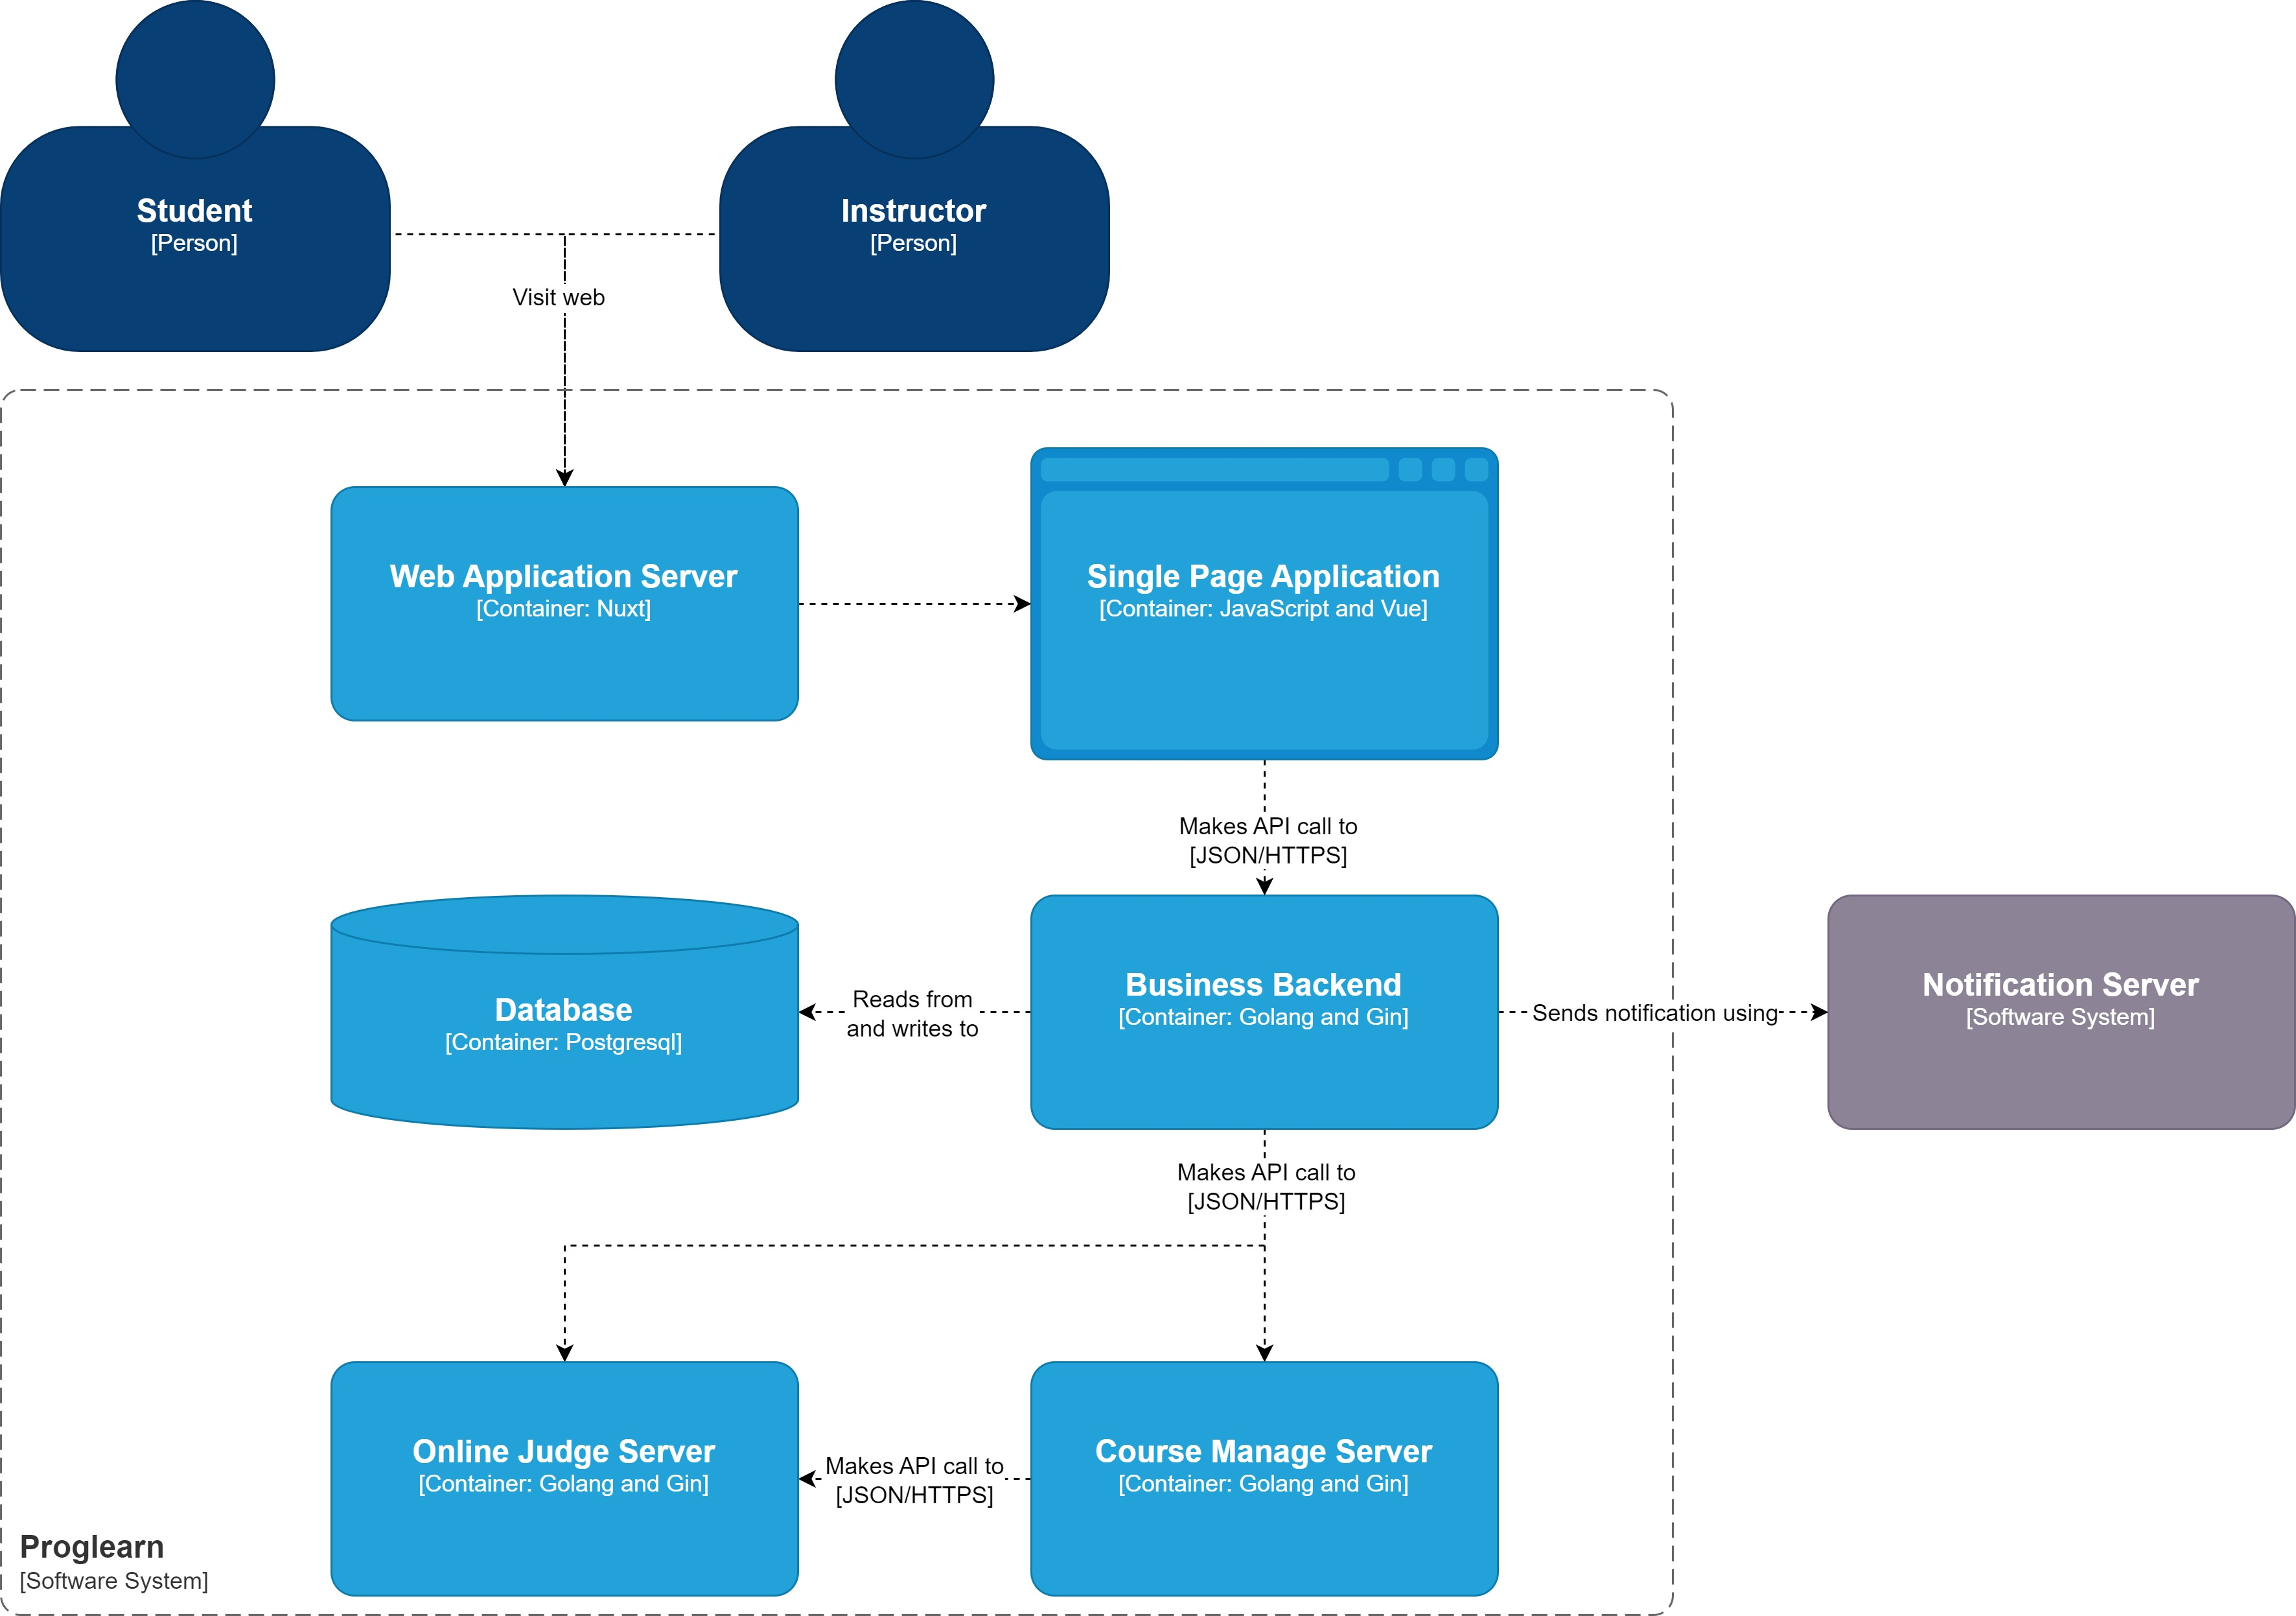
\includegraphics[width=0.65\textwidth]{./img/arc1.jpg}
  %     }
  %     \caption{CAPTION}
  %     \label{arc1}            
  %   \end{subfigure}
  % \end{figure}
\end{enumerate}
\end{document}
